%!TEX root = ../../../super_main.tex

\section{Following the Design Manual}
\label{sec:following_design_guides}
During the fourth sprint, we had a look at the applications we had been working on along with our own design manual and we found that there were some minor problems which required our attention. Some of these problems are described in this section.

\subsection{Incorrect Sidebar}
\label{sec:wrong_sidebar}
Among these minor issues, we found that the side bar in the settings of the \launcher did not conform to our own design manual. It did not use the proper background and did not use a \androidinline{GirafPictogramItemView} in order to display profile images. The \launcher's settings side bar, before and after, can be seen in \figref{fig:launcher_settings_side_bar_before_and_after}. Furthermore, the icons used in the side bar were also updated. The new icons can be seen in \figref{fig:launcher_settings_side_bar_after}. \todo[inline]{TODO START BY THE ONE AND ONLY NIKLAS} Note that these icons cannot be found in the design manual due to lack of time. The next developers of the project should consider to either update the design manual or the icons used. \todo{Skriv at de ikke findes i design manualen.} \todo[inline]{TODO END BY THE ONE AND ONLY NIKLAS}

\begin{figure}[!htbp]
    \centering

    \begin{subfigure}[t]{0.3\textwidth}
        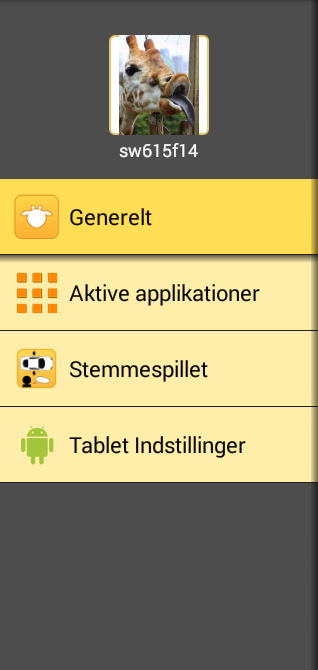
\includegraphics[width=\textwidth]{sprint_four/settings_side_bar_before}
        \caption{Before}
        \label{fig:launcher_settings_side_bar_before}
    \end{subfigure}
    \hspace{5em} 
    \begin{subfigure}[t]{0.3\textwidth}
        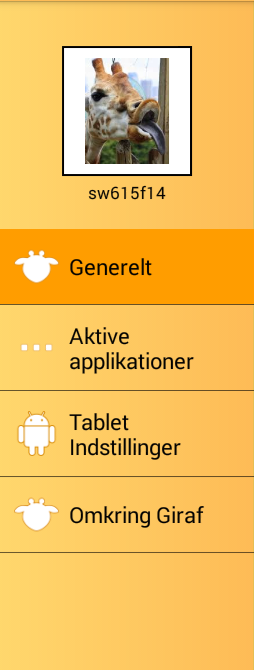
\includegraphics[width=\textwidth]{sprint_four/settings_side_bar_after}
        \caption{After}
        \label{fig:launcher_settings_side_bar_after}
    \end{subfigure}
    
    \caption{Launcher settings side bar before and after}
    \label{fig:launcher_settings_side_bar_before_and_after}
\end{figure}


\subsection{Margin Between Applications}
\label{sec:margin_between_applications}
Both the home screen and settings screen in the launcher was missing spacing between applications in the grid. An example of the problem can be seen in \figref{fig:margin_between_applications_before}. The issue was more pressing in the settings, because the user was able to select the different applications. If the user selected all applications on a screen, it would cause all applications to have an orange background, which might cause the user to be confused as to which applications are actually selected. This problem was corrected by implementing margin between the different applications as seen in \figref{fig:margin_between_applications_after}.  


\begin{figure}[!htbp]
    \centering

    \begin{subfigure}[t]{0.75\textwidth}
        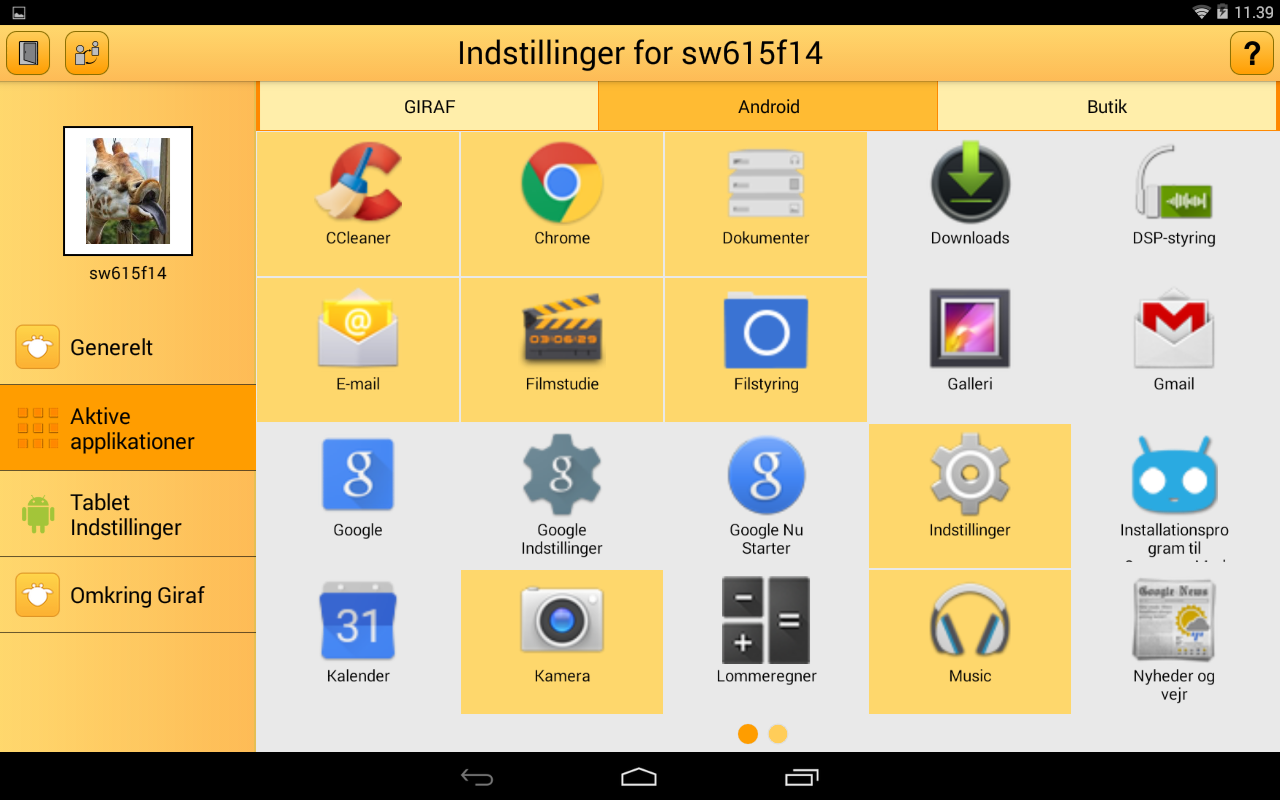
\includegraphics[width=\textwidth]{sprint_four/margin_between_applications_before}
        \caption{Before adding spacing}
        \label{fig:margin_between_applications_before}
        \vspace*{1cm}
    \end{subfigure}
    \begin{subfigure}[t]{0.75\textwidth}
        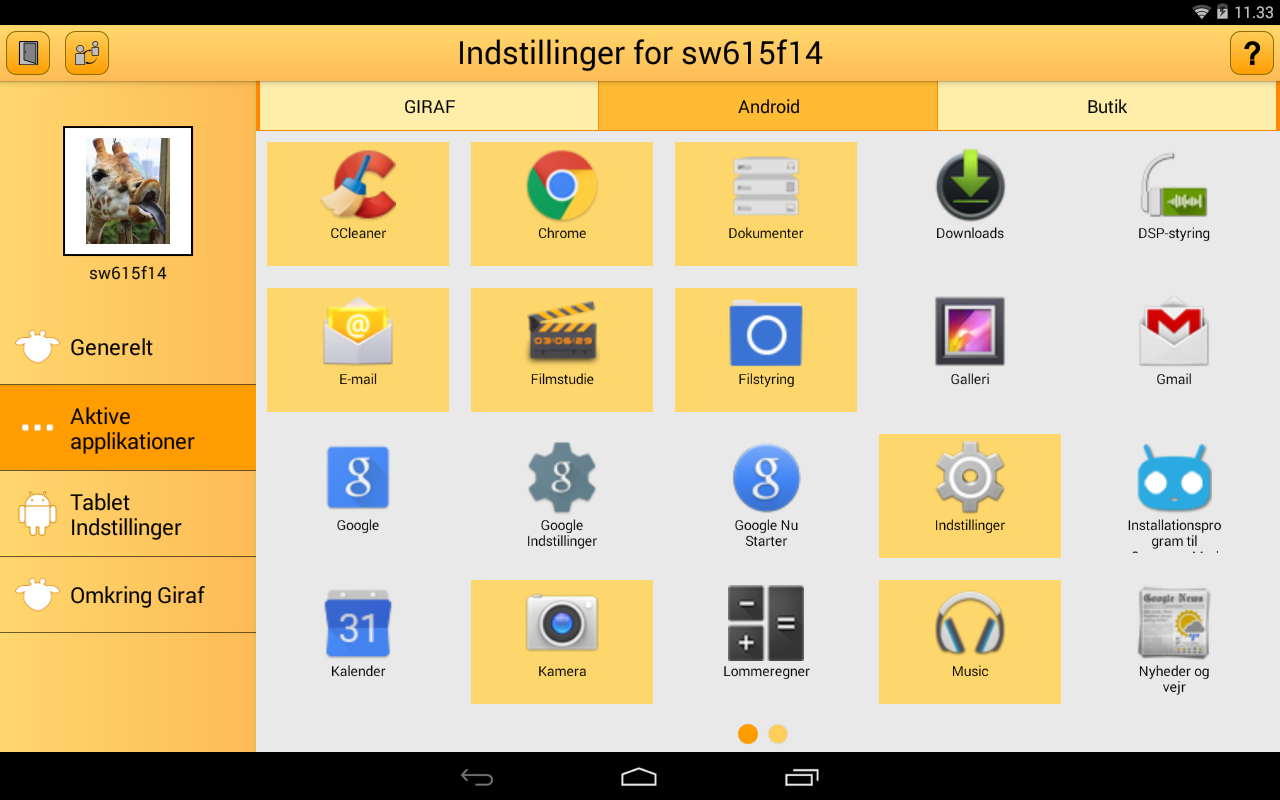
\includegraphics[width=\textwidth]{sprint_four/margin_between_applications_after}
        \caption{After adding spacing}
        \label{fig:margin_between_applications_after}
    \end{subfigure}
    
    \caption{Launcher settings side bar before and after}
    \label{fig:margin_between_applications}
\end{figure}

\FloatBarrier